\chapter{\$1アルゴリズム}
\$Vは\$1の拡張である.そこで本章にて,\$1アルゴリズムを述べる.

\section{特徴}
ユーザが入力した手書きジェスチャは,図\ref{fig:strokes}のように複数の点によって構成され,すでに登録された手書きジェスチャと,それぞれの点を比較することによって,どの手書きジェスチャと一致しているかが判別される.しかしながら,これらの手書きジェスチャを構成する複数の点は,入力に用いられるハードウェアやソフトウェアに依存した速度によってサンプリングされる.それらに加え,人間によって入力される手書きジェスチャにはばらつきがあるため,入力される手書きジェスチャを構成する点の数は入力されるたびに異なる.
そのため,ユーザが入力した手書きジェスチャと,すでに登録された手書きジェスチャを比較するにあたり,手書きジェスチャを構成する点どうしを単純に比較することは困難であると言える.


例えば,図\ref{fig:strokes}の手書きジェスチャは,入力速度によって手書きジェスチャを構成する点の数が異なる例である.それだけでなく,ジェスチャ自体の大きさや向きも異なる.これらは,手書きジェスチャ認識においてジェスチャを比較する上で,1つのハードルとなっている.
これらのような手書きジェスチャによって生じる問題点に対処しつつ,高い認識率を示し,かつどのような開発環境においても実装可能な簡易的なアルゴリズムを実現するために,\$1は以下のような基準に従うようなアルゴリズムの実現を目指した.

\begin{itemize}
\item ハードウェアやソフトウェアのセンシング及び入力する速度などによって変わるサンプリングされる点の数の違いに対してロバストであること.
\item 手書きジェスチャの大きさ,向き,位置に不変な認識をすること.
\item 数学的な高度な知識やテクニックをを必要としないこと~(例えば,逆行列,微分,積分など)
\item 少ないコードによって実装できること.
\item 認識速度が速いこと.
\item ソフトウェア開発者やアプリケーションユーザが,独自に手書きジェスチャを定義できること.
\item N-best listに関して,高い識別能力を示すスコアを示すこと.
\item 図\ref{fig:stroke_1}のような単一ストロークからなる手書きジェスチャを認識するにあたり,HCI分野において多く用いられる既存の複雑な手書きジェスチャ認識アルゴリズムと比べても,高い認識率を示すこと.
\end{itemize}

ここで,N-best listとは,N個の学習データそれぞれに対する入力データとの類似度を降順に並べたものであり,N-best listの1番目と2番目のスコアの差が大きいほど,高い識別能力を示していると言える.

次に,これらの基準に従うように開発された\$1のアルゴリズムを述べる.
アルゴリズムは大きく4つのステップから構成される.


\section{\$1アルゴリズムの4つのステップ}
4.1節において述べた基準を満たすために,入力データ及び学習データは4つのステップを経た後に比較される.
4つのステップは,リサンプル,向きと大きさの正規化,位置の正規化,類似度を高くするための最適な角度の選定からなる.

\subsection{リサンプル}
前節において述べたように,手書きジェスチャを構成する点の数は,ハードウェアやソフトウェアのセンシング及び入力する速度などによって変わる.特に,入力速度の違いによる点の数の違いは顕著である~(図\ref{fig:strokes}).

\begin{figure} [!h]
\centering
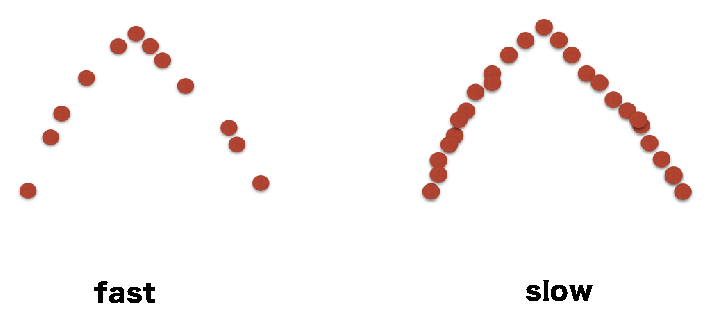
\includegraphics [width=0.8\columnwidth]{img/strokes.eps}
\caption{複数の点から構成されるストローク.同じストロークでも,入力される速度によって点の数が異なる.}
\label{fig:strokes}
\end{figure}

点の数が違うことにより,入力データと学習データの手書きジェスチャを構成する点を互いに比較することが困難となっている.そこで,図\ref{fig:resample}に示すようにN個の等間隔に並ぶ点にリサンプルする.N個の点にリサンプルすることは,生のデータを扱うことと比べて正確なデータを扱っているとは言えず認識精度が落ちる可能性があるが,入力データと学習データ双方の手書きジェスチャの点の数が等しくなるため,容易に互いの対応する点を比較できる.

\begin{figure} [!h]
\centering
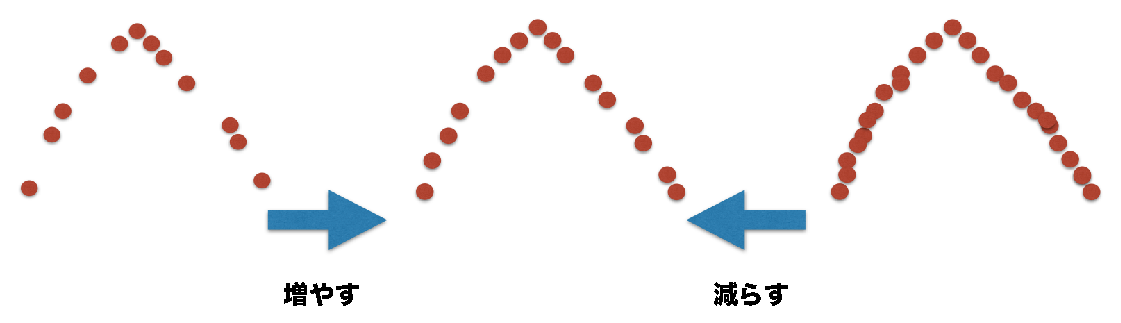
\includegraphics [width=0.8\columnwidth]{img/resample.eps}
\caption{リサンプリングの例.点の数が異なる同じジェスチャも,同じ点の数へとリサンプリングされる.}
\label{fig:resample}
\end{figure}

リサンプルすることは,既存の手書きジェスチャ認識アルゴリズムにおいても用いられている~\cite{Plamondon:2000:OOH:331097.331275, Tappert:1990:SAO:83123.83137, Kristensson:2004:SLV:1029632.1029640, Zhai:2003:SWS:642611.642630, Tappert:1982:CSR:1664966.1664979}.
%\$1はこれらのアルゴリズムを採用するとともに,これらのアルゴリズムとは違い向きに不変なアルゴリズムを提供する.また,
%手書きジェスチャを構成する点の数をリサンプルすることなく実行可能なDTWと比較している.

%N個の等間隔に並ぶ点にリサンプルする方法を図に示す.
%\TODO{リサンプルの仕方を図で説明}

また,リサンプルされる点の数Nは,32$\leq$N$\leq$256の場合,N=64の場合に認識率,認識速度双方において高いパフォーマンスが得られることも\$1において報告されている.

\subsection{向きと大きさの正規化}
リサンプルされた手書きジェスチャの向きを``indicative angle''として定義する.indicative angleとは図\ref{fig:orientation}のように,手書きジェスチャの書き始めの一番最初の点の座標,手書きジェスチャを構成する点全てによる中心座標,0度方向によって形成される角度である.そして,indicative angleに沿って,全てのジェスチャを回転させる.これにより,ジェスチャは向きが正規化される.

\begin{figure} [!h]
\centering
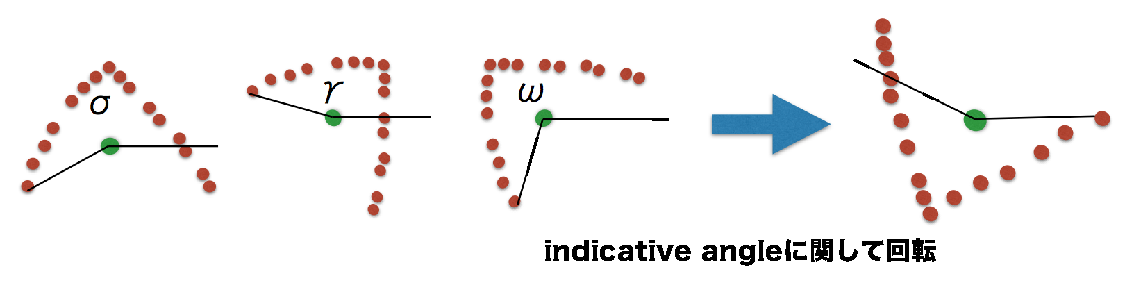
\includegraphics [width=0.8\columnwidth]{img/orientation.eps}
\caption{向きに正規化する例.向きが異なったとしても,同じ向きになるように回転する.}
\label{fig:orientation}
\end{figure}

向きによって正規化されたジェスチャの大きさを``boundingbox''として定義する.boundingboxとは図\ref{fig:size}のように,ジェスチャに隣接するような矩形である.全てのジェスチャについて,boundingboxをある一定の大きさの矩形に正規化することによって,ジェスチャは大きさが正規化される.

\begin{figure} [!h]
\centering
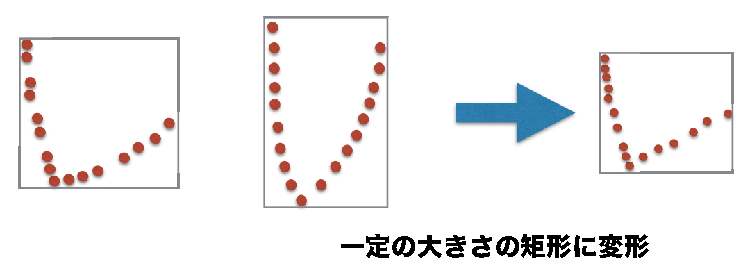
\includegraphics [width=0.7\columnwidth]{img/size.eps}
\caption{大きさに正規化する例.大きさが異なったとしても,同じ大きさになるように変形する.}
\label{fig:size}
\end{figure}

\subsection{位置の正規化}
向きと大きさによって正規化されたジェスチャの位置をジェスチャを構成する全ての点による中心座標として定義する~(図\ref{fig:position}における緑色の点).全てのジェスチャについてこの中心座標を(0, 0)へと移動させることによって,位置が正規化される.

\begin{figure} [!h]
\centering
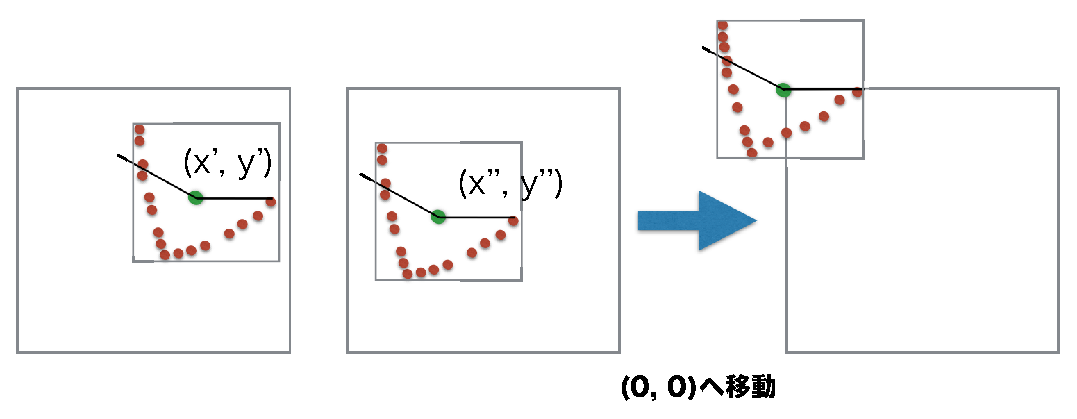
\includegraphics [width=0.8\columnwidth]{img/position.eps}
\caption{位置に正規化する例.位置が異なったとしても,同じ位置になるように移動する.}
\label{fig:position}
\end{figure}

\subsection{類似度を高くするための最適な角度の選定}
リサンプルされた2つの手書きジェスチャ構成する点について,1つずつ対応する点どうし比較するにあたり,$1^\circ$ずつ手書きジェスチャを回転させながら,最も類似度が高くなるような角度を見つけた上で,類似度を算出する方法~\cite{Kara:2005:ITS:1652319.1652712}がある.しかしながらこの方法は認識のために膨大な時間を要することになる.全ての学習データの数が30くらいの場合そのような方法でも十分な速度によって認識することが可能であるが,\$1は黄金分割探索~\cite{Press:1992:NRC:148286}を用いることによって最も類似度が高くなるような角度を求める.
黄金分割探索とは,単峰関数~(極値が1つしかない関数)において,極値を求めるための方法~(局所探索法)のうち効率的な方法の1つであり,極値が存在することが自明な範囲において極値を逐次的に求める方法である.

例えば図\ref{fig:golden}において,$f(x)$の関数があり,極小値$f(x')$を求める時に,$x1$と$x3$の間に極値が存在することが自明な時に,その範囲内に存在する$f(x2)$を求める.この時$x2$は$(x2 - x1) : (x3 - x2)$が黄金比~(1 : $\frac{1+\sqrt{5}}{2}$)となるように設定する.これが黄金分割探索と言われる所以であり,常に3点~(この場合$x1$, $x2$, $x3$)が存在する.その後広い区間~(この場合$x2$と$x3$の間)において,同様に黄金比によって分割し新たな$f(x4)$を得る.この時,$f(x4a)$ならば,極小値は$x1$と$x4$の間に存在するため,新たな3点は$x1$, $x2$, $x4$となる.$f(x4b)$ならば,極小値は$x2$と$x3$の間に存在するため,新たな3点は$x2$, $x4$, $x3$となる.このように,極小値が存在する範囲を徐々に狭めていくことによって,効率よく極値を求めることができる.

\begin{figure} [!h]
\centering
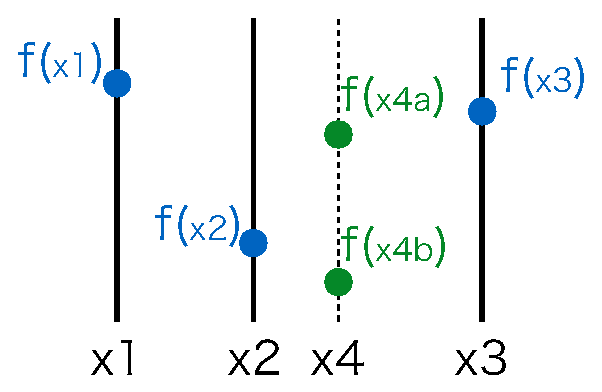
\includegraphics [width=0.6\columnwidth]{img/golden.eps}
\caption{黄金分割探索によって,極値を求める例.}
\label{fig:golden}
\end{figure}

\$1の場合,480個の手書きジェスチャにおいて,$\pm45^\circ$の範囲において極小値が存在することが発見され,極小値が存在する範囲が$2^\circ$になるまで黄金分割探索を行う.この時,入力データに類似する学習データが存在する場合あるいは存在しない場合においても,10ステップ後には極小値が求められることが発見された.

局所探索法の1つである山登り法~\cite{Park:2009:SFA:1464526.1465112,Department94prototypeand}を黄金分割探索の代わりに用いる場合,480個の手書きジェスチャにおいて,類似するジェスチャの場合およそ7.2ステップ後に極小値を求めることができるが,類似しないジェスチャの場合はおよそ53.5ステップ後に極小値が求められることが発見された.つまり学習データが10ずつ存在する16種類の手書きジェスチャ=160個のジェスチャにおいて,黄金分割探索は160$\times$10 = 1600ステップ必要であるのに対し,山登り法は7.2$\times$10 + 53.5$\times$150 = 8097ステップ必要であり,およそ80.2\%もの計算量の節約となっている.

このように,類似度を高くするための最適な角度を黄金分割探索によって効率的に求めることによって,認識速度の向上を実現している.

以上の4ステップをまとめ,入力データと学習データそれぞれを比較するまでの過程を図\ref{fig:onedoller_flow}に示す.
\begin{figure} [!h]
\centering
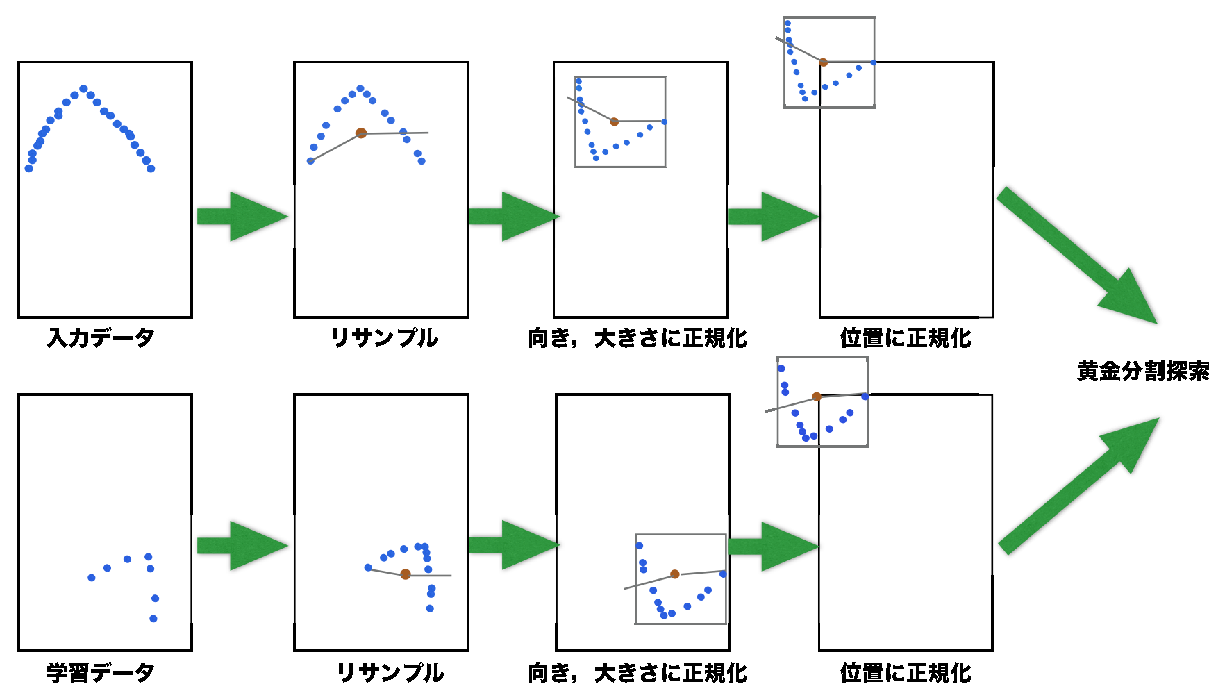
\includegraphics [width=0.9\columnwidth]{img/onedoller_flow.eps}
\caption{\$1アルゴリズムにおいて4つのステップを経て,入力データと学習データが比較されるまでの流れ.}
\label{fig:onedoller_flow}
\end{figure}

\section{類似度計算}
前節までの4ステップによって得られた入力データと学習データの最終的な類似度は式~(4.1)によって表される.
\begin{equation}
score = 1 - \frac{d}{\frac{1}{2}\sqrt{size^2 + size^2}}
\end{equation}
ここで,$d$は対応する点どうしのユークリッド距離の全ての点に関する平均値であり,$size$は大きさに正規化するに用いられる矩形~(正方形)の1辺の長さである.

\section{制約}
\$1は,手書きジェスチャを,大きさ,向き,位置に正規化することによってアルゴリズム全体を簡潔化したり,それぞれについてロバストな認識を可能にし認識率の向上を実現した.しかしながら,このことが原因により,幾つかの制約が存在する.

\begin{itemize}
\item 手書きジェスチャを大きさ,向き,位置によって識別しない.
\item 直線のような1次元の手書きジェスチャを認識することができない.
%\item 手書きジェスチャを入力する速度による識別ができない.
\end{itemize}


「手書きジェスチャを大きさ,向き,位置によって識別しない」ことに関しては,それぞれについて正規化しないようにアルゴリズムを変えることによって識別することが可能となる.しかしながら,正規化しないことにより,正規化しないものに関してはロバスト性が低下するため,結果的に認識率の低下を招く恐れがある.

「直線のような1次元の手書きジェスチャを認識することができない」ことに関しては,向き,大きさに関して正規化した際に図\ref{fig:line}のように,ストロークを構成する各点が分散してしまうためである.

\begin{figure} [!h]
\centering
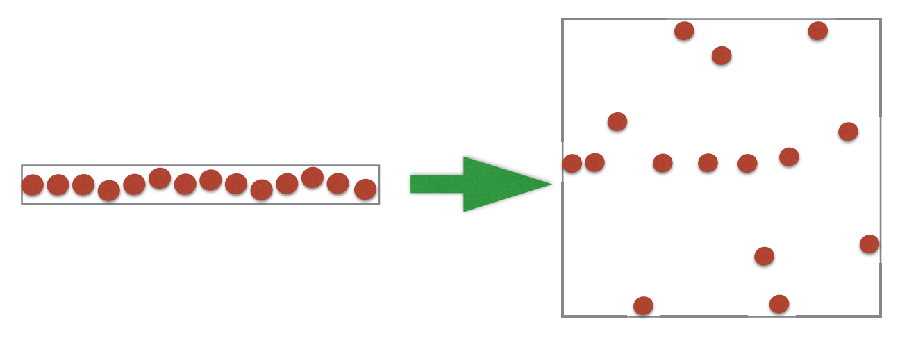
\includegraphics [width=0.8\columnwidth]{img/line.eps}
\caption{\$1が1次元の手書きジェスチャを認識できない理由.向き及び大きさに正規化することによって,ストロークを構成する各点はまばらになってしまう.}
\label{fig:line}
\end{figure}

\$Vは,これらの問題点を解決したアルゴリズムである.

%「手書きジェスチャを入力する速度による識別ができない」ことに関しては,入力速度の要素を特徴量として用いることによって識別可能となる.例えば,Rubine~\cite{Rubine:1991:SGE:122718.122753}は速度を特徴量として用いている.このように認識に用いる特徴量が複数存在する場合,用いる特徴量を適切に選択できれば,つまり,認識に本当に必要な特徴量のみを用いて,認識には必要のない特徴量を選択できれば,認識率の高い手書きジェスチャ認識アルゴリズムとなる.しかしながら,一般的に手書きジェスチャ認識アルゴリズムに関する深い知識がない限り,そのような適切な選択は困難である.\$1は,識別可能な特徴量が少ないが,そのようなわずらわしさを一切省いたアルゴリズムとなっている.



